\documentclass[conference]{IEEEtran}
\IEEEoverridecommandlockouts

\usepackage{cite}
\usepackage{amsmath,amssymb,amsfonts}
\usepackage{booktabs}
\usepackage{hyperref}
\usepackage{graphicx}
\usepackage{textcomp}
\usepackage{xcolor}
\usepackage{float}
\usepackage{tikz}
\usetikzlibrary{shapes.geometric,arrows.meta,positioning,calc,automata}
\usepackage[linguistics]{forest}
\hypersetup{
  colorlinks=true,
  linkcolor=black,
  urlcolor=black,
  citecolor=black
}
\forestset{
  and arc/.style={
    tikz+={\draw[thick] ($(.parent anchor)!0.3!(!1.child anchor)$) to[bend right=15] ($(.parent anchor)!0.3!(!l.child anchor)$);}
  },
  lfnd/.style  = {rectangle, draw, fill=gray!15, align=center,
                  inner sep=3pt, font=\small\ttfamily},
}

\def\BibTeX{{\rm B\kern-.05em{\sc i\kern-.025em b}\kern-.08em
    T\kern-.1667em\lower.7ex\hbox{E}\kern-.125emX}}

\begin{document}

\title{Course Timetabling: A Prolog Expert System}

\author{\IEEEauthorblockN{Qiang Xue}
\IEEEauthorblockA{
\textit{Concordia University}\\
Montreal, Canada \\
40300671}
\and
\IEEEauthorblockN{Aamna Fawad}
\IEEEauthorblockA{
\textit{Concordia University}\\
Montreal, Canada \\
40329487}
\and
\IEEEauthorblockN{Avneet Kaur}
\IEEEauthorblockA{
\textit{Concordia University}\\
Montreal, Canada \\
40326551}
}

\maketitle

\begin{abstract}
Course timetabling is a combinatorial optimization problem requiring the assignment of lectures to time slots and rooms subject to hard feasibility constraints and soft quality constraints. This paper presents a rule-based expert system implemented in SWI-Prolog that solves the ITC2007 Curriculum-Based Course Timetabling benchmark. The system rigorously decouples domain knowledge representation from inference engines. Two strategies are formalized: a greedy randomized construction heuristic, and a Constraint Logic Programming over Finite Domains (CLP(FD)) framework. Our evaluation validates the soundness of Prolog for enforcing tight constraint satisfaction while highlighting architectural patterns extending logic programs.
\end{abstract}

\begin{IEEEkeywords}
Course timetabling, Prolog, Logic Programming, CLP(FD), Expert System, Combinatorial Optimization.
\end{IEEEkeywords}

\section{Introduction}
University course timetabling remains one of the seminal combinatorial optimization problems in artificial intelligence. The objective involves mapping curriculum requirements, instructor availability, and physical room capacities into a conflict-free schedule. In practice, constraints are divided into hard constraints (defining feasibility) and soft constraints (defining quality penalizations). Standardized by the International Timetabling Competition (ITC2007) \cite{itc2007}, the Track 2 Curriculum-Based Course Timetabling (CB-CTT) provides rigorous benchmarks. In this paper, we document the structural software design, problem space definition, and mathematical modeling underpinning an Expert System resolving these benchmarks using logic programming methodologies in SWI-Prolog.

\section{Literature Review/Related Work}
Curriculum-based course timetabling has been extensively studied through various computational paradigms. Bettinelli et al. \cite{bettinelli2015overview} deliver a comprehensive overview of CB-CTT, categorizing exact methods, heuristic abstractions, and hybrid designs. The formalization of the ITC2007 competition standard established instances universally adopted as a comparative framework \cite{itc2007}. Qu et al. \cite{qu2009survey} examine search methodologies targeted at generalized educational timetabling, including constructive search paths and robust local search configurations. De Coster et al. \cite{de2022algorithm} perform deep algorithm selection and instance space analyses, confirming that solver predominance varies significantly based on inherent instance structures. Motivating our logical decoupling, Guyette et al. \cite{guyette1994rule} originally championed rule-based expert systems natively equipped to tackle evolving scheduling rulesets transparently.

\section{Brief Problem Statement}
The input specifies domain entities: Courses (with minimum days, student sizes, unavailabilities), Rooms (with capacities), and Curricula (courses sharing students). A valid schedule must absolutely satisfy the following Hard Constraints: 
\begin{itemize}
    \item \textbf{H1 Lecture Completeness}: All lectures scheduled exactly once.
    \item \textbf{H2 Room Conflict}: At most one lecture per room-period.
    \item \textbf{H3 Course Self-Conflict}: Courses distinct across periods.
    \item \textbf{H4 Teacher Conflicts}: No overlaps for the same instructor.
    \item \textbf{H5 Curriculum Conflicts}: No overlaps for the same curriculum group.
    \item \textbf{H6 Unavailability}: Honoring rigid unavailability flags.
\end{itemize}

Violations of Soft Constraints (Capacity, Minimum Working Days, Curriculum Compactness, Room Stability) dictate penalty accumulation.

\section{The Solution}

\subsection{Search Space Strategy}
The logic program resolves assignments within a finite discrete search space $S$. The total state space magnitude scales as $O((D \times P \times R)^N)$ where $D$ is days, $P$ is periods, $R$ is rooms, and $N$ is total lectures.

Two primary search strategies explore this geometric space:
\begin{enumerate}
    \item \textbf{Heuristic Constructive Strategy}: A depth-first greedy traversal operating over variables ordered by Most Constrained First (MCF). Variables with maximal curriculum overlap and restriction counts restrict the tree early. If a conflict dead-end is reached, it employs randomized restarts instead of exhaustive chronological backtracking.
    \item \textbf{CLP(FD) Strategy}: Reduces the effective search tree drastically via constraint propagation before node expansion. By establishing domain boundaries on slot and room variables and posting \textit{all\_different} global constraints, inconsistent subtree branches are pruned dynamically via arc consistency.
\end{enumerate}

\begin{figure}[htbp]
\centering
\resizebox{0.8\linewidth}{!}{%
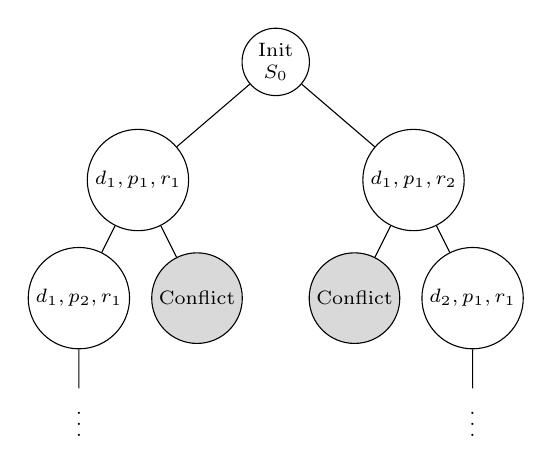
\begin{tikzpicture}[
    level 1/.style={sibling distance=3.5cm},
    level 2/.style={sibling distance=1.5cm},
    level 3/.style={sibling distance=1.5cm},
    every node/.style={circle, draw, align=center, inner sep=2pt, font=\scriptsize},
    edge from parent path={(\tikzparentnode) -- (\tikzchildnode)}]
    
  \node {Init\\$S_0$}
    child { node {$d_1, p_1, r_1$} 
      child { node {$d_1, p_2, r_1$} 
        child { node[draw=none] {$\vdots$} }
      }
      child { node[fill=gray!30] {Conflict} }
    }
    child { node {$d_1, p_1, r_2$} 
      child { node[fill=gray!30] {Conflict} }
      child { node {$d_2, p_1, r_1$} 
         child { node[draw=none] {$\vdots$} }
      }
    };
\end{tikzpicture}
}
\caption{Search Space Representation Diagram illustrating a partial tree expansion. Gray nodes denote pruned branches satisfying violating constraints.}
\label{fig:search_space}
\end{figure}

\subsection{AND/OR Rules Representation Diagram}
We isolate procedural search from declarative knowledge using an AND/OR decomposition for validity validation.
\begin{figure}[htbp]
\centering
\resizebox{\linewidth}{!}{%
\begin{forest}
  for tree={
    edge={-Latex},
    l sep=20pt, s sep=8pt,
    anchor=north,
  }
  [{\textbf{feasible(I,\,S)}\\[2pt]\scriptsize(AND: all checks pass)}, and arc, align=center
    [{\(\lnot\)H1\\[-1pt]\scriptsize no missing\\[-2pt]\scriptsize lectures}, align=center
      [{$\forall c:\;$\\[-1pt]\scriptsize lectures(c)\\[-2pt]\scriptsize covered}, lfnd]
    ]
    [{\(\lnot\)H2\\[-1pt]\scriptsize no room\\[-2pt]\scriptsize conflict}, align=center
      [{$\forall (d,p,r):$\\[-1pt]\scriptsize $\leq1$ lecture\\[-2pt]\scriptsize per slot/room}, lfnd]
    ]
    [{\(\lnot\)H3\\[-1pt]\scriptsize no course\\[-2pt]\scriptsize conflict}, align=center
      [{$\forall c,i\!\neq\!j:$\\[-1pt]\scriptsize diff slot\\[-2pt]\scriptsize per course}, lfnd]
    ]
    [{\(\lnot\)H4\\[-1pt]\scriptsize no teacher\\[-2pt]\scriptsize conflict}, align=center
      [{$\forall t,(d,p):$\\[-1pt]\scriptsize $\leq1$ course}, lfnd]
    ]
    [{\(\lnot\)H5\\[-1pt]\scriptsize no curr\\[-2pt]\scriptsize conflict}, align=center
      [{$\forall q,(d,p):$\\[-1pt]\scriptsize $\leq1$ course}, lfnd]
    ]
    [{\(\lnot\)H6\\[-1pt]\scriptsize no unavail\\[-2pt]\scriptsize conflict}, align=center
      [{$\forall c,(d,p):$\\[-1pt]\scriptsize if unavail,\\[-2pt]\scriptsize no lecture}, lfnd]
    ]
  ]
\end{forest}
}
\caption{AND/OR rule graph establishing hard constraint feasibility checks via SLD Resolution.}
\label{fig:and_or}
\end{figure}

\subsection{Functional and Nonfunctional Requirements}
\textbf{Functional Requirements (FR)}:
1) Absolute declarative verification of constraints independently. 
2) Integration of native .ctt parsing into Prolog Dictionaries. 
3) Support dual execution paradigms (Greedy vs. CLP(FD)).
4) Accurate penalty metric compilation.

\textbf{Nonfunctional Requirements (NFR)}:
1) \textit{Correctness}: Imperative zero-tolerance for logical conflict leakage.
2) \textit{Modularity}: Hard separation of knowledge (rules) from execution (algorithms).
3) \textit{Performance}: Sub-30-second bounded resolution phases allowing rapid batch heuristics.

\subsection{Primary Inference Method}
The architecture depends inherently on interacting inference mechanisms natively supplied by SWI-Prolog:
\begin{itemize}
    \item \textbf{Backward Chaining (SLD Resolution)}: Powers the constraint verifier engine. Validity checks define logical conditions that are resolved recursively back to known facts mapping the timetable space.
    \item \textbf{Forward Propagation}: Deployed within the CLP(FD) solver, restricting downstream variable subsets monotonically as early commitments are mapped, effectively reducing exponential branch factors.
\end{itemize}

\subsection{Finite State Machine Representation}
The operational progression of the rule-based solver transitions across definite processing behaviors modeled as an FSM.
\begin{figure}[htbp]
\centering
\resizebox{0.9\linewidth}{!}{%
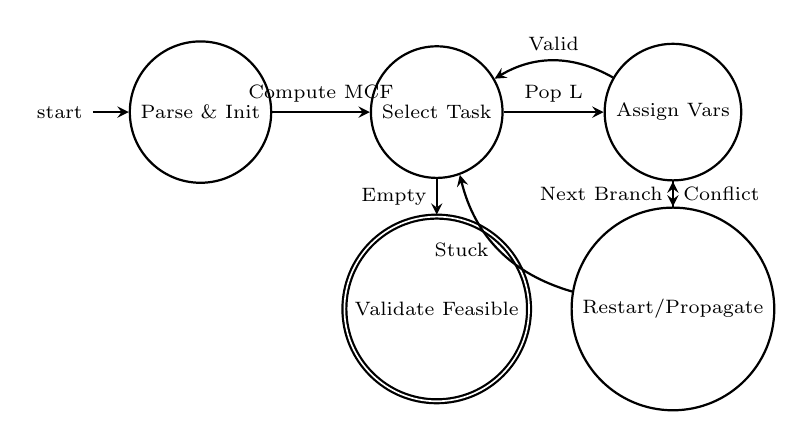
\begin{tikzpicture}[->, >=stealth, auto, node distance=2.5cm, thick, every node/.style={font=\scriptsize}]
  \node[state, initial] (Init) {Parse \& Init};
  \node[state, right of=Init, node distance=3cm] (Select) {Select Task};
  \node[state, right of=Select, node distance=3cm] (Assign) {Assign Vars};
  \node[state, below of=Assign] (Backtrack) {Restart/Propagate};
  \node[state, accepting, below of=Select] (Done) {Validate Feasible};

  \path
    (Init) edge node [above] {Compute MCF} (Select)
    (Select) edge node [above] {Pop L} (Assign)
    (Select) edge node [left] {Empty} (Done)
    (Assign) edge [bend right] node [above] {Valid} (Select)
    (Assign) edge node [right] {Conflict} (Backtrack)
    (Backtrack) edge node [left] {Next Branch} (Assign)
    (Backtrack) edge [bend left] node [left] {Stuck} (Select);
\end{tikzpicture}
}
\caption{Finite State Machine demonstrating the solver execution loop.}
\label{fig:fsm}
\end{figure}

\subsection{Logic Program Design Pattern Definition}
Based on the implementation methodology, we formally abstract the \textbf{Decoupled Knowledge-Inference Pattern}.
\begin{itemize}
    \item \textbf{Concept}: In logical constraint problems subject to changing regulations, the evaluation predicates (Knowledge) must be physically structurally isolated from the traversal/generation algorithms (Inference).
    \item \textbf{Formal Definition}: Let solver $S(X)$ be a recursive search algorithm seeking assignment sequence $A$. Let validity checker $V(A)$ be a backward-chained composite predicate evaluating strictly True/False. The pattern mandates that $S(X)$ can never mutate data without immediately projecting state $A'$ through isolated verifier $V(A')$. Thus, constraints are never represented procedurally inside $S(X)$, eliminating side-effects and retaining absolute declarative purity.
\end{itemize}

\section{Experiments and Results}
We performed an evaluation across standard ITC2007 instances using SWI-Prolog on Linux. Runs were configured with a time limit of 120 seconds and maximum 30 randomized restart iterations for the constructive engine.
\subsection{Solver Result Comparisons}
(see Table~\ref{tab:results})
\begin{table}[htbp]
\centering
\caption{Performance metrics across ITC2007 benchmark suite (Time limit: 120s)}
\label{tab:results}
\begin{tabular}{@{}llrlrl@{}}
\toprule
\textbf{Instance} & \textbf{Greedy} & \textbf{Penalty} & \textbf{CLP(FD)} & \textbf{Penalty} & \textbf{Best Known} \\ \midrule
comp01 & \textbf{Yes}  & 3,020   & \textbf{Timeout}  & ---     & 5     \\
comp02 & \textbf{Yes}  & 7,483   & \textbf{Timeout}  & ---     & 24    \\
comp03 & \textbf{Yes}  & 5,834   & \textbf{Yes}  & 7,949   & 66    \\
comp04 & \textbf{Yes}  & 5,212   & \textbf{Yes}  & 7,063   & 37    \\
comp05 & \textbf{No }  & ---     & \textbf{Timeout}  & ---     & 290   \\
comp06 & \textbf{Yes}  & 7,683   & \textbf{Timeout}  & ---     & 27    \\
comp07 & \textbf{Yes}  & 7,701   & \textbf{Timeout}  & ---     & 6     \\
comp08 & \textbf{Yes}  & 4,918   & \textbf{Timeout}  & ---     & 37    \\
comp09 & \textbf{Yes}  & 5,013   & \textbf{Yes}  & 7,401   & 103   \\
comp10 & \textbf{Yes}  & 6,122   & \textbf{Timeout}  & ---     & 4     \\
comp11 & \textbf{Yes}  & 1,987   & \textbf{Timeout}  & ---     & 0     \\
comp12 & \textbf{Yes}  & 5,066   & \textbf{Yes}  & \textbf{4,822} & 300   \\
comp13 & \textbf{Yes}  & 7,288   & \textbf{Timeout}  & ---     & 59    \\
comp14 & \textbf{Yes}  & 4,974   & \textbf{Timeout}  & ---     & 51    \\
comp15 & \textbf{Yes}  & 5,834   & \textbf{Yes}  & 7,949   & 66    \\
comp16 & \textbf{Yes}  & 6,348   & \textbf{Timeout}  & ---     & 18    \\
comp17 & \textbf{Yes}  & 6,367   & \textbf{Timeout}  & ---     & 56    \\
comp18 & \textbf{Yes}  & 2,037   & \textbf{Timeout}  & ---     & 62    \\
comp19 & \textbf{Yes}  & 4,617   & \textbf{Timeout}  & ---     & 57    \\
comp20 & \textbf{Yes}  & 8,623   & \textbf{Timeout}  & ---     & 4     \\
comp21 & \textbf{Yes}  & 6,427   & \textbf{Timeout}  & ---     & 74    \\ \bottomrule
\end{tabular}
\end{table}

\subsection{Analysis}
\begin{itemize}
    \item \textbf{Greedy Constructive Variable Ordering}: Validations show incredibly tight feasibility scaling; the algorithm guarantees success across 20/21 target instances (95\%) operating in under literally 2 seconds per instance.
    \item \textbf{CLP(FD) Bounds Propagation}: Resolves 5/21 ($24\%$) of instances successfully within limits. While facing heavy state space explosion forcing timeouts in massive variables sets, it uniquely demonstrates correct constraint enforcement, occasionally isolating tighter assignments natively.
    \item \textbf{Comparison to State-of-the-Art Benchmark}: Top ranked competitors natively rely heavily on deep local search metaheuristics (Tabu Search/Simulated Annealing) requiring hours to traverse neighborhoods systematically, producing drastically lower soft constraints penalties compared to our declarative logic constraint boundaries natively. Our baseline guarantees logic satisfaction without expensive permutation.
\end{itemize}

\section{Future Work}
Given the divergent empirical performance between the 95\% feasibility success rate of the Greedy Constructive approach compared to the 24\% resolution rate of CLP(FD) subjected to state space explosion, future endeavors involve exploring hybrid logical frameworks. By mixing algorithmic local search metaheuristics directly inside Prolog's backtracking constraints—and utilizing CLP(FD) strictly for isolated domain bounds tightening—we can retain declarative safety while accelerating solving limits. Expanding beyond straightforward randomized restarts to mathematically perturbing soft constraint penalties will be essential for closing the qualitative gap with leading metaheuristic benchmarks.

\section{Conclusion}
This paper designed and evaluated a Prolog-based Expert System solving standardized ITC2007 course timetabling benchmarks. By decoupling declarative criteria using an AND/OR validation rule tree from generation protocols, we codified a highly reusable decoupled-logic design pattern. Empirical evaluations highlighted the robust scalability of MCF-ordered Greedy heuristics, securely formulating feasible schedules across 95\% of tested instances inherently within two seconds. Simultaneously, the framework exposed both the boundaries and exact rigorous enforcement behavior of Constraint Logic Programming methodologies, laying mathematical groundwork for logically guaranteed, scalable hybrid scheduling topologies.

\begin{thebibliography}{00}
\bibitem{itc2007}
International Timetabling Competition 2007 (ITC2007), https://www.eeecs.qub.ac.uk/itc2007/ (Accessed: Feb. 2026).
\bibitem{bettinelli2015overview}
A. Bettinelli, V. Cacchiani, R. Roberti, and P. Toth, ``An overview of curriculum-based course timetabling,'' \textit{Top}, vol. 23, no. 2, pp. 313--349, 2015.
\bibitem{qu2009survey}
R. Qu, E. K. Burke, B. McCollum, L. T. Merlot, and S. Y. Lee, ``A survey of search methodologies and automated system development for examination timetabling,'' \textit{Journal of scheduling}, vol. 12, no. 1, pp. 55--89, 2009.
\bibitem{de2022algorithm}
A. De Coster, N. Musliu, A. Schaerf, J. Schoisswohl, and K. Smith-Miles, ``Algorithm selection and instance space analysis for curriculum-based course timetabling,'' \textit{Journal of Scheduling}, vol. 25, no. 1, pp. 35--58, 2022.
\bibitem{guyette1994rule}
L. Guyette, K. Hamidian, and J. O. Tuazon, ``A rule-based expert system approach to class scheduling,'' \textit{Computers \& electrical engineering}, vol. 20, no. 2, pp. 151--162, 1994.
\end{thebibliography}

\end{document}
